\documentclass[12pt]{article}
\usepackage[margin=1in]{geometry}
\usepackage{graphicx}
\usepackage{booktabs}
\usepackage{amsmath}
\title{The Effect of Paid Search Advertising on Revenue: \\
A Replication of the eBay Natural Experiment}
\author{Vic Oquendo}
\date{\today}
\begin{document}
\maketitle
\section{Introduction}
This paper examines the causal effect of paid search advertising on eBay's revenue. Firms collectively spend billions of dollars each year on search engine marketing (SEM), yet rigorously measuring its incremental contribution to revenue remains difficult because of endogeneity, selection effects, and the inability to observe counterfactual outcomes. To overcome these challenges, the analysis exploits a natural experiment in which eBay voluntarily suspended its paid search advertisements in a subset of geographic markets.

\section{Experimental Setting}
In 2012, Blake et al. (2014) persuaded eBay to cease bidding on Google AdWords as part of a large-scale field experiment. Of the 210 designated market areas (DMAs) in the United States, 65 were assigned to the treatment group in which paid search was turned off beginning May 22, 2012; the intervention lasted eight weeks. In the treatment group, the indicator \texttt{search\_stays\_on} equals zero, while it remains equal to one in the control group. 

Importantly, the experiment was not a fully randomized trial: the largest DMAs were deliberately excluded from treatment. As a result, the treatment and control groups differ systematically in baseline revenue levels. This imbalance rules out a simple comparison of means and instead motivates the use of a difference-in-differences (DID) design that can net out time-invariant group differences and common time trends.

\section{Data and Figures}
The dataset comprises daily aggregate revenue for all 210 DMAs from April through July 2012. The principal variables are the calendar date, a unique DMA identifier, binary indicators for the post-treatment period and treatment group, and (scaled and shifted) revenue.

\begin{figure}[h]
\centering
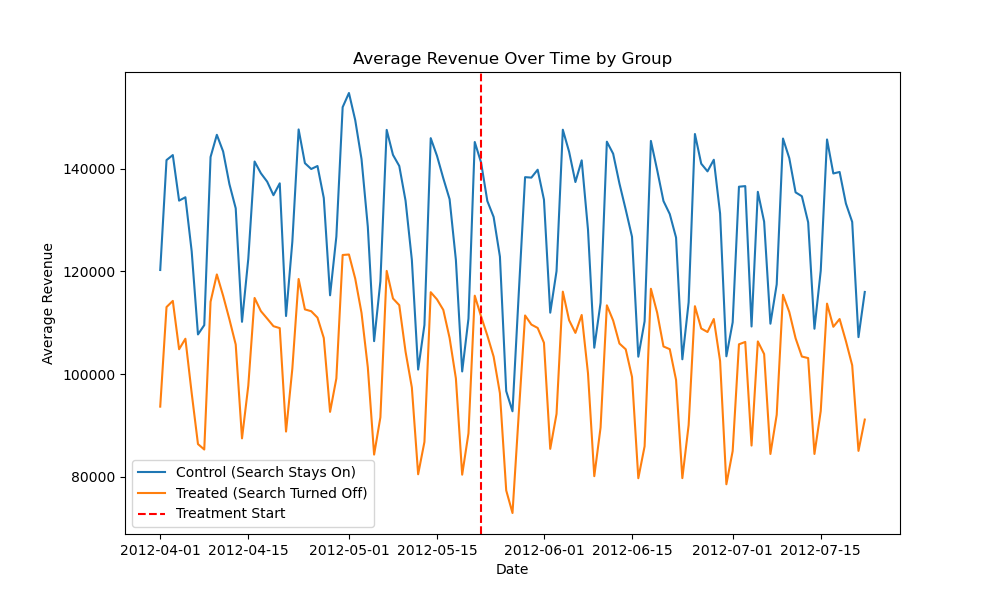
\includegraphics[width=0.85\textwidth]{../output/figures/figure_5_2.png}
\caption{Average revenue for treatment and control DMAs over time.
The dashed line marks May 22, 2012, when SEM was turned off
for the treatment group.}
\label{fig:revenue}
\end{figure}

The control group displays substantially higher average revenue throughout the sample period, consistent with the deliberate exclusion of the largest DMAs from treatment. Both groups nevertheless exhibit nearly identical weekly oscillation patterns driven by day-of-week and holiday effects. At the scale shown, however, any divergence immediately following the May 22 intervention is difficult to discern visually.

\begin{figure}[h]
\centering
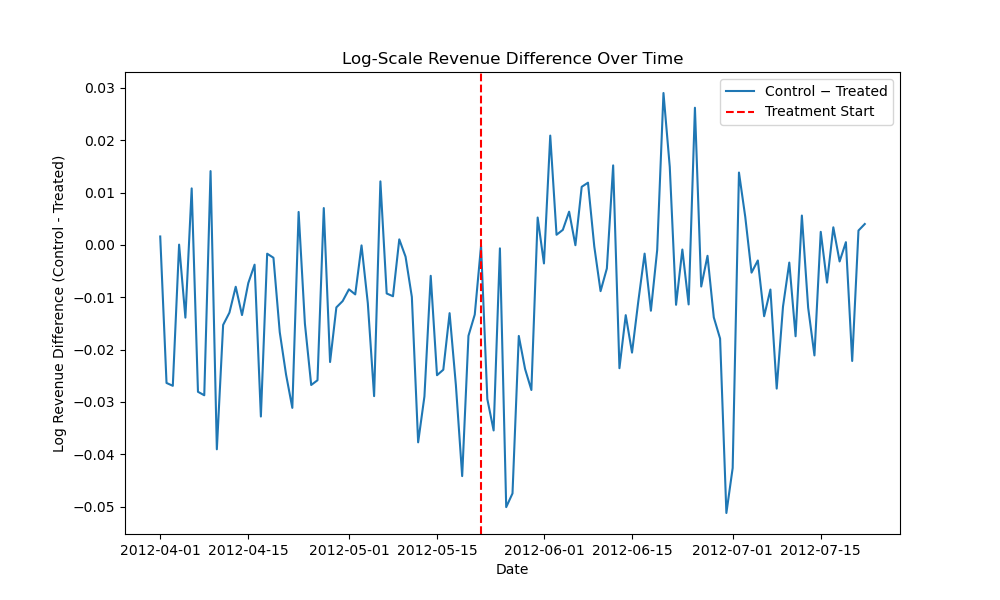
\includegraphics[width=0.85\textwidth]{../output/figures/figure_5_3.png}
\caption{Log-scale average revenue difference between control and treatment
groups over time. The gap appears to increase after May 22.}
\label{fig:logdiff}
\end{figure}

Figure~\ref{fig:logdiff} plots the log ratio of average control-group revenue to average treatment-group revenue. Prior to the intervention the series fluctuates around a stable level; after May 22 the gap widens modestly. Although the visual change is subtle, the pattern is consistent with a small negative effect of paid search and provides the motivation for a formal difference-in-differences test.

\section{Results}
\input{../output/tables/did_table.tex}

The difference-in-differences estimator yields a point estimate of \(\hat{\gamma} = -0.0066\) on the log-revenue scale. Exponentiating gives \(\exp(-0.0066) \approx 0.9934\), which implies that the treatment DMAs lost roughly 0.66 percent of revenue when paid search was turned off. The associated 95 percent confidence interval is \([-0.0175, 0.0043]\), which comfortably contains zero. Consequently the estimated effect is not statistically significant at conventional levels.

Economically, the results indicate that suspending paid search produced a very small---and statistically indistinguishable from zero---decline in eBay's revenue. For a well-known brand such as eBay, the great majority of potential customers appear to locate the site through organic search regardless of whether paid advertisements are present.

\section{Conclusion}
The difference-in-differences analysis finds a small and statistically insignificant effect of paid search advertising on eBay's revenue. This exercise successfully replicates the central qualitative conclusion of Blake et al. (2014). Several caveats should be kept in mind: the revenue series is scaled and shifted (not the actual dollar figures), the treatment assignment was not fully randomized, and the specification uses a simple DID model without additional covariates or fixed effects. Nevertheless, the finding carries important implications for marketing practice: even large, sophisticated advertisers may substantially overstate the incremental return on search-engine marketing expenditures when they rely on observational rather than experimental evidence.
\begin{thebibliography}{9}
\bibitem{blake2014}
Blake, T., C. Nosko, and S. Tadelis (2014).
``Consumer Heterogeneity and Paid Search Effectiveness: A Large-Scale Field Experiment.''
\textit{Econometrica}, 83(1): 155--174.
\bibitem{taddy2019}
Taddy, M. (2019).
\textit{Business Data Science}. McGraw-Hill, Chapter 5.
\end{thebibliography}
\end{document}
